
Figure 1: The common concern of three fields

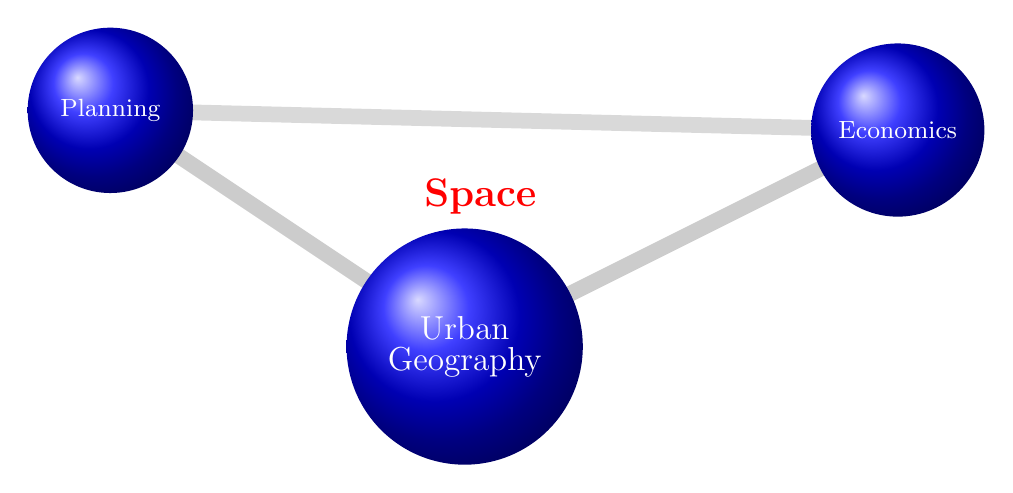
\begin{tikzpicture}{scale=.5}
% find color cotrol for ball. Tind way to stop line short of node
\coordinate (planning) at (-5,1);%PREFACE
\coordinate (economics) at (5,.75);%
 \coordinate (geography) at (-.5,-2); %history
\coordinate (finance) at (0,5); %

\draw [line width=2mm, black!15, ] (planning)--(economics);
\draw [line width=2mm, black!20, ] (geography)--(economics);
\draw [line width=2mm, black!20, ] (geography)--(planning);

%\draw [line width=2mm, black!25, ] (geography)--(finance);
%\draw [line width=2mm, black!20, ] (planning)--(finance);
%\draw [line width=2mm, black!20, ] (finance)--(economics);

\node [circle,shading=ball, minimum width=2.1   cm, white, align=center] (ball) at (planning) {Planning};
\node [circle,shading=ball, minimum width=2.2cm, white, align=center] (ball) at (economics) {Economics};
\node [circle,shading=ball, minimum width=3 . cm, white, align=center] (ball) at (geography)[text width=2cm] {\large Urban\\ Geography};

%\node [circle, shading=ball, minimum width=2.4cm, white, align=center] (ball) at (finance)[text width=2cm] {Finance};

\node at (-.3,-.1) [red] {\Large \textbf{Space}};
\end{tikzpicture}

\vspace{2cm}


Figure 2 with names

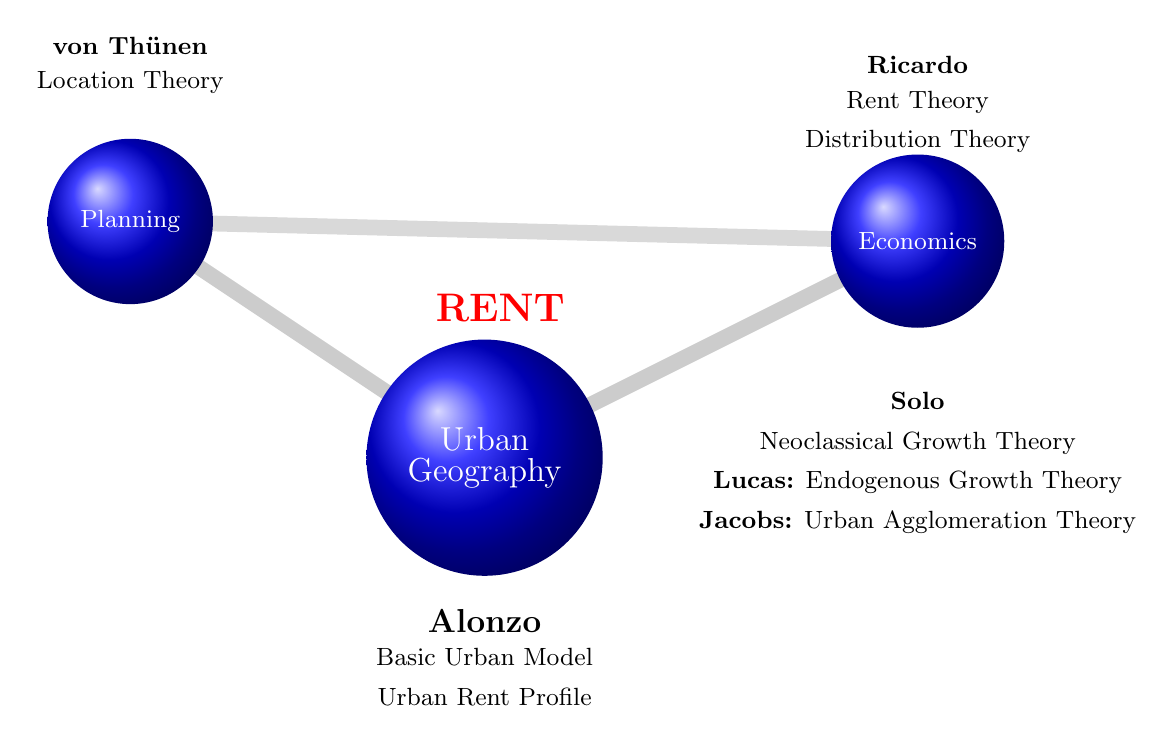
\begin{tikzpicture}{scale=.5}
% find color cotrol for ball. Tind way to stop line short of node
\coordinate (planning) at (-5,1);%PREFACE
\coordinate (economics) at (5,.75);%
 \coordinate (geography) at (-.5,-2); %history
\coordinate (finance) at (0,5); %

\draw [line width=2mm, black!15, ] (planning)--(economics);
\draw [line width=2mm, black!20, ] (geography)--(economics);
\draw [line width=2mm, black!20, ] (geography)--(planning);

%\draw [line width=2mm, black!25, ] (geography)--(finance);
%\draw [line width=2mm, black!20, ] (planning)--(finance);
%\draw [line width=2mm, black!20, ] (finance)--(economics);

\node [circle,shading=ball, minimum width=2.1   cm, white, align=center] (ball) at (planning) {Planning};
\node [circle,shading=ball, minimum width=2.2cm, white, align=center] (ball) at (economics) {Economics};
\node [circle,shading=ball, minimum width=3 . cm, white, align=center] (ball) at (geography)[text width=2cm] {\large Urban\\ Geography};

%\node [circle, shading=ball, minimum width=2.4cm, white, align=center] (ball) at (finance)[text width=2cm] {Finance};

\node at (-.3,-.1) [red] {\Large \textbf{RENT}};

% new stuff
\node at (planning) [above=2cm] {\textbf{von Th\"unen}};
\node at (planning) [above=1.5cm] {Location Theory};

\node at (economics) [above=2cm] {\textbf{Ricardo}};
\node at (economics) [above=1.5cm] {Rent Theory};
\node at (economics) [above=1.0cm] {Distribution Theory};

\node at (economics) [below=1.8cm] {\textbf{Solo}};
\node at (economics) [below=2.3cm] {Neoclassical Growth Theory};
\node at (economics) [below=2.8cm] {\textbf{Lucas:} Endogenous Growth Theory};
\node at (economics) [below=3.3cm] {\textbf{Jacobs:} Urban Agglomeration Theory};


\node at (geography) [below=1.8cm] {\textbf{\large Alonzo}};
\node at (geography) [below=2.3cm] {Basic Urban Model};
\node at (geography) [below=2.8cm] {Urban Rent Profile};
\end{tikzpicture}



Figure 3: space and value

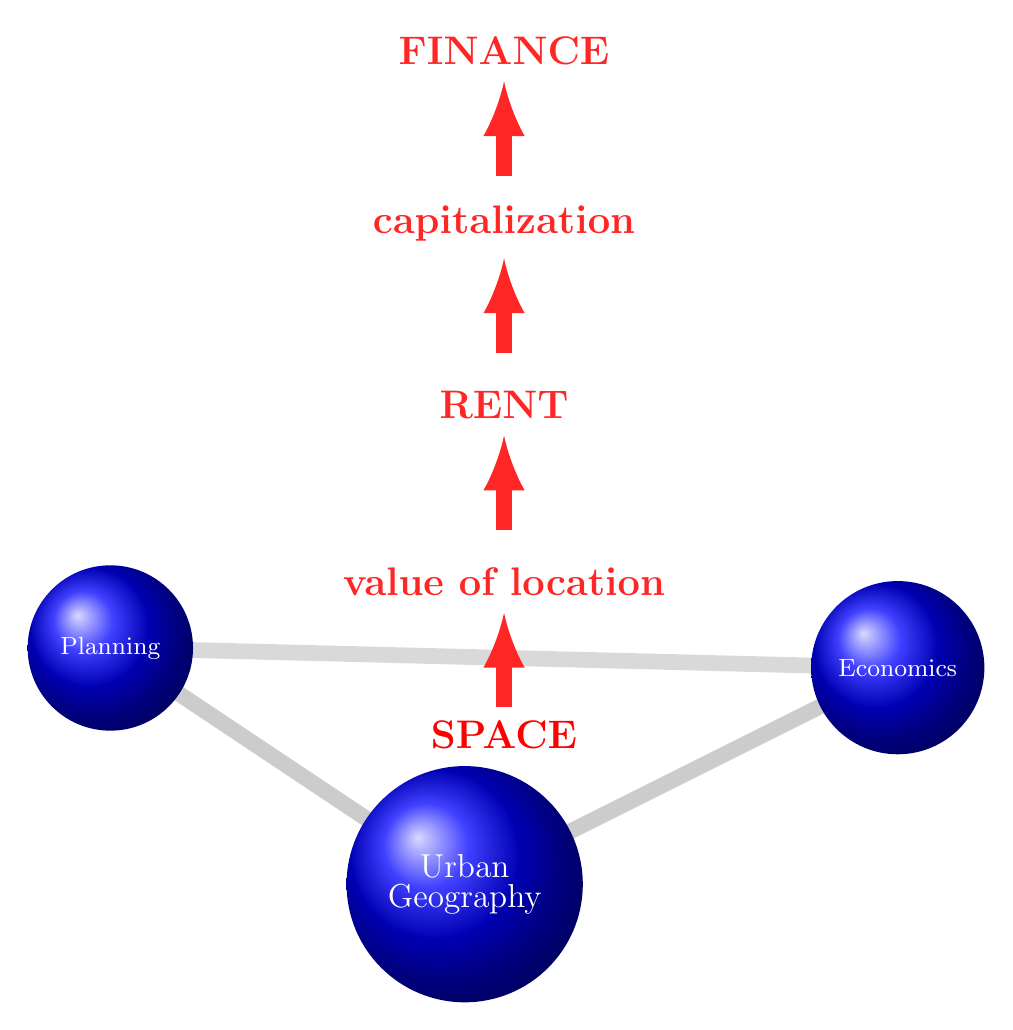
\begin{tikzpicture}{scale=.5}
% find color cotrol for ball. Tind way to stop line short of node
\coordinate (planning) at (-5,1);%PREFACE
\coordinate (economics) at (5,.75);%
 \coordinate (geography) at (-.5,-2); %history
\coordinate (finance) at (0,5); %

\draw [line width=2mm, black!15, ] (planning)--(economics);
\draw [line width=2mm, black!20, ] (geography)--(economics);
\draw [line width=2mm, black!20, ] (geography)--(planning);

%\draw [line width=2mm, black!25, ] (geography)--(finance);
%\draw [line width=2mm, black!20, ] (planning)--(finance);
%\draw [line width=2mm, black!20, ] (finance)--(economics);

\node [circle,shading=ball, minimum width=2.1   cm, white, align=center] (ball) at (planning) {Planning};
\node [circle,shading=ball, minimum width=2.2cm, white, align=center] (ball) at (economics) {Economics};
\node [circle,shading=ball, minimum width=3 . cm, white, align=center] (ball) at (geography)[text width=2cm] {\large Urban\\ Geography};

%\node [circle, shading=ball, minimum width=2.4cm, white, align=center] (ball) at (finance)[text width=2cm] {Finance};
\draw [line width=2mm, red!85, -latex ] (0, 7)--++(0,1.2)node[above=-.1] {\Large \textbf{FINANCE}};
\draw [line width=2mm, red!85, -latex ] (0, 4.75)--++(0,1.2)node[above=-.1] {\Large \textbf{capitalization}};
\draw [line width=2mm, red!85, -latex ] (0, 2.5)--++(0,1.2)node[above=-.1] {\Large \textbf{RENT}};
\draw [line width=2mm, red!85, -latex ] (0, .25)--++(0,1.2)node[above=-.1] {\Large \textbf{value of location}};
\node at (0,-.1) [red] {\Large \textbf{SPACE}};
\end{tikzpicture}





\vspace {2cm}
Figure 4 with finance

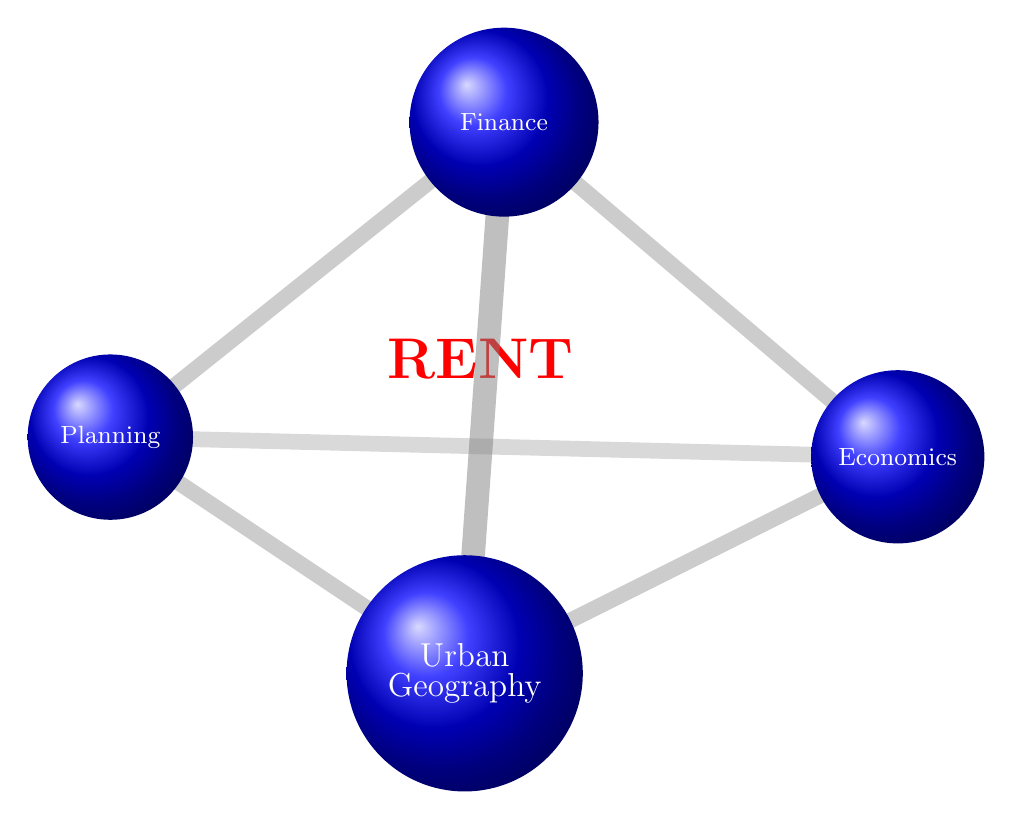
\begin{tikzpicture}{scale=.5}
% find color cotrol for ball. Tind way to stop line short of node
\coordinate (planning) at (-5,1);%PREFACE
\coordinate (economics) at (5,.75);%
 \coordinate (geography) at (-.5,-2); %history
\coordinate (finance) at (0,5); %

\draw [line width=2mm, black!15, ] (planning)--(economics);
\draw [line width=2mm, black!20, ] (geography)--(economics);
\draw [line width=2mm, black!20, ] (geography)--(planning);

\node at (-.3,2) [red] {\huge \textbf{RENT}};

\draw [line width=3mm,  black!50,opacity=.5 ] (geography)--(finance);
\draw [line width=2mm, black!20, ] (planning)--(finance);
\draw [line width=2mm, black!20, ] (finance)--(economics);

\node [circle,shading=ball, minimum width=2.1   cm, white, align=center] (ball) at (planning) {Planning};
\node [circle,shading=ball, minimum width=2.2cm, white, align=center] (ball) at (economics) {Economics};
\node [circle,shading=ball, minimum width=3 . cm, white, align=center] (ball) at (geography)[text width=2cm] {\large Urban\\ Geography};

\node [circle, shading=ball, minimum width=2.4cm, white, align=center] (ball) at (finance)[text width=2cm] {Finance};


\end{tikzpicture}


\vspace {2cm}
Figure 4 with finance

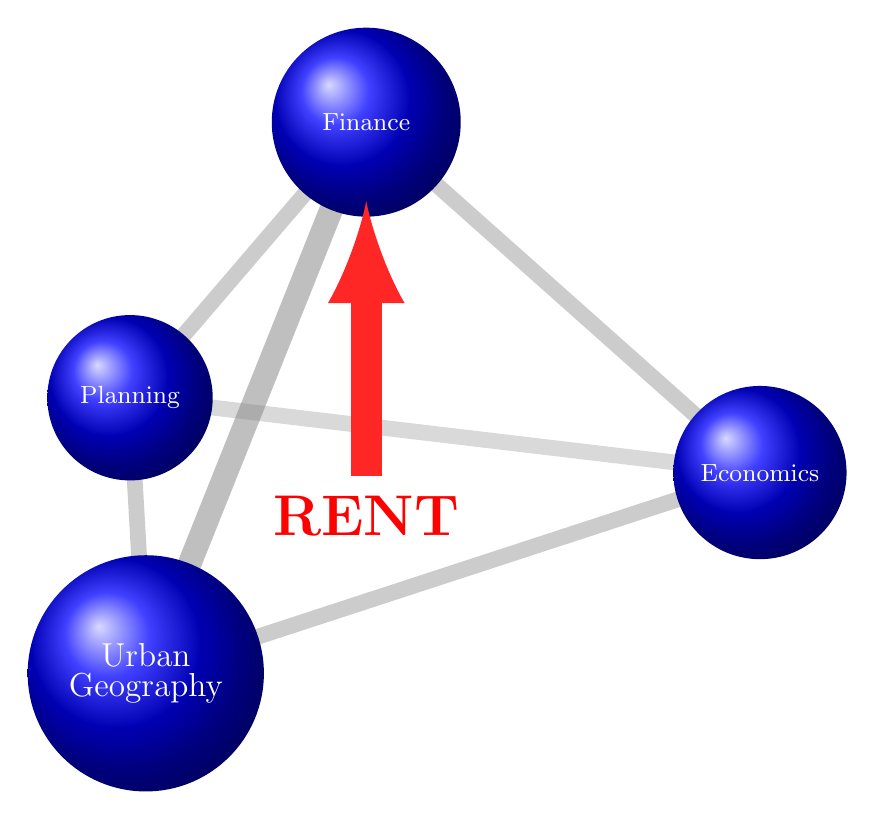
\begin{tikzpicture}{scale=.5}
% find color cotrol for ball. Tind way to stop line short of node
\coordinate (planning) at (-3,1.5);%PREFACE
\coordinate (economics) at (5,.55);%
 \coordinate (geography) at (-2.8,-2); %history
\coordinate (finance) at (0,5); %

\draw [line width=2mm, black!15, ] (planning)--(economics);
\draw [line width=2mm, black!20, ] (geography)--(economics);
\draw [line width=2mm, black!20, ] (geography)--(planning);

\node at (.0,0) [red] {\huge \textbf{RENT}};

\draw [line width=3mm,  black!50,opacity=.5 ] (geography)--(finance);
\draw [line width=2mm, black!20, ] (planning)--(finance);
\draw [line width=2mm, black!20, ] (finance)--(economics);

\node [circle,shading=ball, minimum width=2.1   cm, white, align=center] (ball) at (planning) {Planning};
\node [circle,shading=ball, minimum width=2.2cm, white, align=center] (ball) at (economics) {Economics};
\node [circle,shading=ball, minimum width=3 . cm, white, align=center] (ball) at (geography)[text width=2cm] {\large Urban\\ Geography};

\node [circle, shading=ball, minimum width=2.4cm, white, align=center] (ball) at (finance)[text width=2cm] {Finance};
\draw [line width=4mm, red!85, -latex ] (0, .5)--(0,4);


\end{tikzpicture}



\vspace{2cm}

\section{Financialization and Urban Land Rents}
%BASED ON Financialization_of_the_Housing_Market.tex

Financialization is the process by which financial institutions, markets, etc., increase in size and influence. More specifically it is the process by which future streams of revenue and speculative gains are systematically captured by individuals and institutions with financial assets. Financialization of the housing market is the increasing control of the stock of urban land and housing in order to capture the scarcity rent generated by the people of the city.  

Mortgages, for example, are a financial instrument that allows lenders to  participate in housing purchases in the present in exchange for a future flow of payments.  The mortgage does not create housing, but it enables the prospective buyer to become the nominal owner of an asset that produces a stream of benefits. The stream of benefits from secure housing near a source of income generally greatly exceeds a buyer's current assets. The mortgage enables the  transfer of ownership because it makes it possible to transfer the rights to the future income of the buyer to the mortgage holder who then, in effect, is the actual owner until the terms of the mortgage are fulfilled.  If the mortgagee fails make those payments the mortgage holder  takes over the asset. 

The mortgage itself is both an financial instrument that enables a purchase and a financial asset that can be bought and sold. When we consider urban housing, it is the right to future income generated by capital, labour and the the city itself through the agglomeration effects that drive productivity. It is an instrument that indirectly captures a share of the urban rents. As productivity rises, wages rise, rents rise, property prices rise and mortgages rise. 

About 80\% of Canadian homes are owner-occupied and about a third of the  value of the homes is held as mortgages. Approximately two-thirds of the net land rents associated with housing therefore accrue to owner occupiers. {\color {red}CHECK THESE NUMBERS } 

For urban theory and policy formation it is important to distinguish between financial instruments that enable production of real assets and instruments like the mortgage that facilitate the transfer of real assets. Housing developers borrow to purchase land for development and builders borrow to finance construction. While important, the financial instruments involved are not driving the financialization of housing.  The size of the loans involved is affected by the amount of land purchased and the potential rents earned by that land, the degree of non-occupant ownership is not affected.






  a productive asset is acquired as a financial asset it remans productive. %African land or land in Northern Ontario acquired by holding companies may even be made more productive. 
The goal of such investments, however, is generally to achieve a capital gain over time. Financial analysis is essentially about rates of return on financial capital invested. The opportunity for capital gains  attracts financial capital to the housing market.%Financial managers have no interest is n in assets that are not expected to increase in value. 
\footnote{.} 

Financialization of urban housing benefits  a globally distributed rentier class of urban landholders. We will make this more explicit below the incentive structure deriving the further financialization of the housing market.

\section{Literature on theory and evidence}
{\color{red}There is substantial evidence that the financialization of urban housing is underway in Canadain cities

PROVIDE EVIDENCE 	mention theories?}


Two questions arise when we observe growing participation of global capital in the urban housing system: 
\begin{enumerate}
\item How far will the financialization of urban land go? 
\item That are the implications for the urban economy and the welfare of the urban population? 
\end{enumerate}

We can demonstrate  that  in the absence of policy interventions, differential access to finance capital ensures that capital owners acquire an increasing share of urban land over time and capture the growing  land rents  from urban productivity growth. Growing wealth inequality emerges within a simple, widely accepted model of the urban land market. In the limit,  urban residents are tenants, and new residents  without capital do  not receive any of the increases in rents arising from the growing productivity of the city. 

%The first question therefore is reduced to which capital holders will increase their share of urban land and whether there is any reason to expect the process of financialization process to stop or reverse itself.




\section{The incentives for financialization}%\label{Sec:RentAndClass}

  

%Instead, drawing on the ideas of Jane Jacobs, Lucas proposes the city as the unit of analysis .Lucas, Robert (1990), "Why Doesn't Capital Flow from Rich to Poor Countries?," American Economic Review Papers and Proceedings v. 80, no. 2 (May) pp. 92-96.  
%Jacobs, Jane  (1969), The Economy of Cities (New York: Random House).  
% The Death and Life of Great American Cities \cite{Jacobs61}




\section{The rate of return on a property purchase}


ADD TABLE WITH VARIABLE DEFINITIONS
 
 In this section we develop a model of the return to investment in urban housing/land. We'll assume that all agents are speculating on potential capital gains as well as on the use values they get from a property.  We will also assume that the use value is captured by the stream of rental values, whether a home is owner occupied or  held by an investor as a financial asset. To keep the analysis simple without loss of generality we will consider a one-period investment.
 
 The speculator  invests a down payment, $D$, and gets back at time $T$ the  increased price $(1+\dot p)P_0$, plus rents, minus any costs and minus the mortgage with interest.\footnote{We have applied this model to explore the effect of a vacancy tax in Beirut.  Fort that analysis we  added a use-value, $U$ in place of rent for expatriate owners to represent using the property - say one month a year - when they are not renting the property and a \textbf{vacancy tax}, $T$ at rate $t$ to affect the speculator's  decision. \cite{Al-Shihabi}}


\begin{eqnarray*}
V  	&=& capital\ gain - Interest\ due  	+ Rent  - operating\ cost -taxes\\
% 	&=& \delta P_T-D \qquad \qquad \quad - (1+\delta r)M \quad	 + R  	-C\\
% 	&=& \delta P _T \qquad-(P_0-M) \quad- (1+\delta r)M 	 + R  	-C\\
%	&=& \delta (1+\dot p)  P_0 -(P_O -M)  -(1+\delta r)mP_0  + R  -C\\
%	&=& \delta (1+\dot p)  P_0 -P_O + M \qquad -(1+\delta r)mP_0  + R -C\\
%	&=&( \delta (1+\dot p)-1)  P_0  + mP_0 \quad -(1+ \delta r)mP_0  + (\rho-\kappa)P_0\\	
%	&=& \left(  \delta (1+\dot p)-1    + m \quad - m(1+\delta r)  + (\rho-\kappa)\right)P_0\\'
%	&=& \left(  \delta (1+\dot p)-1    + m \quad - m-\delta rm  + (\rho-\kappa)\right)P_0\\
&=& \delta(P_T- (1+r)M) \qquad \qquad 	 + R  	-C   - T\\
&=& \delta((1+\dot p)  P_0- (1+r)mP_0)   + \rho P_0  	-\kappa P_0 - tP_0\\
&=&( \delta((1+\dot p)  - (1+r)m) \ + \rho   	-\kappa -t) P_0
\end{eqnarray*}

This is the  net present value of buying, and selling after one period. It has  6 exogenous parameters, $\delta, \dot p, r, m, \rho, \kappa$ and $t$.   Operating revenue and costs $\rho, \kappa$ and $t$ are expressed as  present values. Both the  share of the price  that can be mortgaged, $m$, and the interest rate  and $r$ are functions of the agent's wealth. $\delta$ may be correlated with wealth as well. 

The rate of return $v$ is the value of the gain, $V$, divided by  the size of the downpayment, $D$. 
%The rate of return is $v = \frac{V}{D}$. %For expat investors, we get a \textbf{decision rule}:\begin{enumerate}
%\item  if $v \geq a$ (with some private use?) with no rent,  don't bother renting. 
%\item If $v(no\ rent\ and\ tax) < a\geq v(with\ rent)$,  then  rent. 
%\item If $ v(with\ rent) \le a $,  then sell 
%\end{enumerate}\
\begin{eqnarray}
v&=&( \delta((1+\dot p)  - (1+r)m) \ + \rho   	-\kappa - t ) \frac{P_0}{D}   \nonumber\\
		&=&( \delta((1+\dot p)  - (1+r)m) \ + \rho   	-\kappa - t ) \frac{P_0}{P_0-mP_0}   \nonumber\\
		&=&\frac{ \delta(1+\dot p  - (1+r)m) \ + \rho   	-\kappa - t } {1-m} \label{Eqn:DecisionRule}
\end{eqnarray}






%%%%%%%%  VVVVVVVVVVVVVVVVVVVVVVV   This section May 18 to cut?  V
%%%%%%%%  ^^^^^^^^^^^^^^^^^^^^^^^^^^^^^^^  This section May 18 to cut?  V

%\begin{enumerate}
%
%\item  the buyer and seller calculate the value of the property  differently. 
%
%\item  the  buyer and seller may have different expectations of the path of prices and therefore the stream of rents.
%%There are two standard ways that expectations are modelled
%%	\begin{enumerate}
%%	\item \textbf{Adaptive expectations.} Expectations are largely based on what has happened in the past. 
%%	Under normal conditions most people people have relatively weak incentive to get forecasts about inflation correct, and lack the resources and time to purchase expert advice. 
%%	Recent price trends are easily available and likely to be the main source of  information.
%%	\item     \textbf{Rational expectations.} Expectations are based on a model of the future economy. 
%%International investors and banks employ economists and other experts to  forecast prices, exchange rates, and trends in the economy.
%%	\end{enumerate} 
%\end{enumerate}
% Why would  discount rates differ between identical workers? Buyers and sellers are not identical in wealth, obviously. 
%%We could implement the first  explanation either by generating expectational errors based on functional class or wealth. 

%As expected
%\begin{enumerate}
%\item A large $m$ magnifies the return. (downpayment is smaller)
%\item A lower mortgage interest rate increases the return because of interest on the mortgage
%\item A lower discount rate $\delta$ reduces the subjective rate of return
%\item Higher expected price appreciation increases the attractiveness of investment
%\item Higher rents makes the unit more profitable if rents are being collected
%\item Lower costs increase profits
%\item Lower tax rates decrease holding costs and increase the value of the investment
%\end{enumerate}
The implications of Equation~\ref{Eqn:DecisionRule} are significant for the evolution of the urban land market and class structure. They suggest strongly that large wealth-holders will get higher expected and actual rates of return on land than those with  lower wealth holdings,\footnote{Case and Schiller ``%The ratio of construction costs to price, changes in adult population and
 ... increases in real per capita income all are positively related to excess returns or price changes over the subsequent year.''} and that the managers of large pools of capital will have an even greater advantage. 
 
 Make list of effects variable by variable. describe derivatives
 
Consistent with the empirical evidence, net returns for investment are increasing with wealth. 
%
%\begin{enumerate}
%\item Given the  common rule that mortgage payments cannot exceed some fraction of disposable income, the wealthy will be able borrow larger amounts and at lower interest rates that the less wealthy. At any distance from the centre they will be able to make a higher bid.
%
%\item The cost of capital is known to differ for rich and poor. Say, for example, the cost of borrowing, $r_i$ for agent $i$ if the base lending rate is $\bar{r}$
% \[ r_i = (A + B \frac{\bar{W}}{W_i})\bar r\]
%where $\bar{W}$ is mean wealth and $W_i$ is individual wealth. Figure~\ref{Fig:BorrowingCost} illustrates the effect.\footnote{Fr\'ed\'erick Demers found that the response of housing investment to interest rates has become more pronounced over time. Modelling and Forecasting Housing Investment: The Case of Canada,  Research Department, Bank of Canada, Ottawa, Ontario, Canada K1A 0G9 fdemers@bankofcanada.ca} 
%
%\begin{figure}[htbp]
%\begin{center}
%\chapter{SAPriceOfCapital}

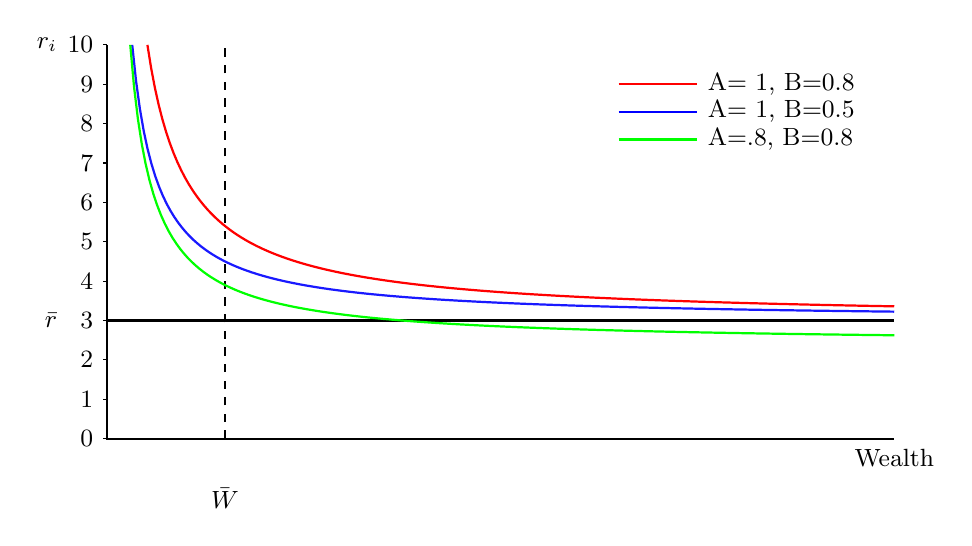
\begin{tikzpicture}[scale=.5]
%\def\bndmax{5}        %https://tex.stackexchange.com/questions/68462/filling-a-complex-region-with-tikz
%\def\bndmin{0.2}
\def \Y {10}  % height of y axis pecent
\def \W {20}  % length  of x axis
\def \Wbar {3} % jmeam wealth
\def \omega {3}
\def \A {1}  %was .5
\def \B {.5}
%Equation   \[ r_i = (A + .5 \frac{\bar{W}}{W_i})\omega\]
\def \Wmin{.63}  %This sets the lower limit fo the 
\def \Wmin{(\B*\Wbar)/(\Y/\omega-\A)} %function to keep in in bounds
	
\tikzset{func/.style={thick,color=blue!90}}	

\draw [thick] (0,\Y)node[left=.5cm]{$r_i$} -- (0,0)--(\W,0)node[below]{Wealth};  	% Axes
\draw [thick] (0,\omega)node[left=.5cm]{$\bar r$} -- (\W,\omega);  	% Axes
\draw [thick,dashed] ( \Wbar,0)node[below=.5cm]{$\bar{W}$} -- (\Wbar,\Y);  	% Axes

\foreach \yi in {0,...,\Y} \draw (0,\yi)--(-.1,\yi)node[left]{\small$\yi$};

\draw[func,domain=\Wmin:\W] plot [samples=200] (\x,{(\A+\B*\Wbar/\x)*\omega});
\def \A {.8}
\draw[func,domain=\Wmin:\W, green] plot [samples=200] (\x,{(\A+\B*\Wbar/\x)*\omega});

\def \A {1}
\def \B {.8}
\draw[func,domain=\Wmin:\W, red] plot [samples=200] (\x,{(\A+\B*\Wbar/\x)*\omega});

\draw [red,  thick](13, 9)--(15,9)node [right, black] {\small A=\ 1,\ B=0.8};
\draw [blue,  thick](13, 8.3)--(15,8.3)node [right, black] {\small A=\ 1,\ B=0.5};
\draw [green, thick](13, 7.6)--(15,7.6)node [right, black] {\small A=.8, B=0.8};
 \end{tikzpicture}
% Figure of cost of borrowing
%\caption{Borrowing cost for  $A=1$  $B=0.5$ (blue);  $A=1$  $B=0.8$ (red);  $A=.8$  $B=0.8$ (green);}
%%\caption{Hypothetical wealth-dependent borrowing cost}
%\label{Fig:BorrowingCost}
%\end{center}
%\end{figure}%
%
%\item If agents discount at their borrowing rate, wealthier agents may have a lower subjective rate of time preference and therefore value properties more highly. 
%\end{enumerate}

The implication is that those with more capital will be at an advantage in the urban housing  market. Tax treatment of income and capital gains as well as interest deductability will influence Equation~\ref{Eqn:DecisionRule}'s strength and who benefits most. 

There are some additional implications

%\begin{enumerate}
%\item  expecting greater price appreciation raises expected profitability. The wealthy and financial corporations  are likely to have better price forecasts than  the occasional home buyer.
%\item higher expected  rents may result from expecting greater price appreciation raises expected profitability or greater willingness to raise rents for tenants
%\item There may be scale economies in maintenance  of rented housing
%\item There may be opportunities to shelter income with land held for investment (speculative) purposes
%\end{enumerate}

These items suggest that financial corporations may have advantages relative to individual investors. Combined with better access to capital and interest deductability, it is reasonable to expect that financial corporations, which essentially pool the purchasing power of wealth holders, increasingly dominate urban land markets. %A recent report claimed 15\% of Tioron0's land transa

In the limit it appears that wage income will never be sufficient to support home ownership in growing cities. 
Overall, this suggests rising housing prices are not a bubble because speculation decouples use-value from price setting. %


These observations about  the rate of return on urban capital raise a set of very interesting issues.  


\begin{itemize}
\item The effect of increasing the urban workforce is to increase the marginal products of  both capital and labour throughout the urban economy. This premium on production in cities is positive when $\Lambda'$ is greater than zero.
 \item  As long as $\Lambda'>0$ cities will  grow, potentially leading to the ``catastrophic agglomeration''  that has been noted in other models.  %(\cite{FujitaKrugmanVenables, BaldwinMartin, Krugman1991, Gurwitz2019}).  City size could be bounded, in which case the city system would grow by increasing the number of cities. This appears to depend on the model features and parameters. 
\item Cities will draw investment away from rural and remote areas.
\item Cities will draw labour away from rural and remote areas. 
\item Even in competitive markets capital captures  scale benefits until an entry equilibrium is achieved.
\item Landowners  capture the agglomeration benefits that are not dissipated in transportation costs.
\end{itemize}

These appear to be features of the economy we observe.


\section{The long-run evolution of complex urban systems}

It is clear that cities city systems and city economies are complex systems. Complex systems are sensitive to scale and tend to generate emergent properties over time. In the history of cities we discern a series of transitions arising out of growing size and complexity. There is no reason to  think that evolution has stopped. In fact our analysis has focussed on a significant transition that is currently underway. The transformation of cities as humans become an urban species has had a series of stages, each of which was tied to production technologies and largely determined social relations of the period.

Early cities were built on 
 




DOES THIS GO TO THE MODEL CHAPTER?

The model is we employ consistent with the theories of Ricardo and Henry George in locating the ground of urban exploitation and class in the capacity to extract social surplus through land ownership, and differs from the standard Marxian analysis in its reliance on access to financial capital rather than control of productive physical capital. The paper concludes that given existing land ownership patterns which encourage speculative investment, housing prices must rise and income inequality must increase. 



We  incorporate Jacobs-style agglomeration economies (\cite{Beaudry:2009ua, Panne:2004vb, JacobsEofC})  similar to the way the  Solo-Swan model incorporates  labour-augmenting technical change using a simple Cobb-Douglas production function.  We bypass the complexity of modelling firms  by allowing population increases  to directly increase urban wage premium.\footnote{The transmission of productivity increases arising from agglomeration effects  to the urban wage through firms, can be modelled in many ways. The agglomeration effects are external to the firm and therefore likely to be unexpected. If  firms underestimate the marginal product of labour, labour productivity will be greater than expected, output will be higher than planned output, and revenue and profits will therefore be higher than expected. Excess demand will attract more productive capital which in turn will demand more labour,  Rising labour demand drives up the wage. The agglomeration effect driving growth is essentially a public good in which individual firms will under-invest. This raises an policy challenge that we leave for others.} %, It is straightforward to compute the rate of excess return for  this model. 
%We insert the production function  into a standard Alonso-style model of a city economy (\cite{Alonso64}). 
In the background, individual firms have decreasing returns, but the presence of agglomeration economies external to firms but internal to the city gives the urban economy as a whole increasing returns to scale. \footnote{These effects can be large. Irwin and Klenow  studied learning in chip production focusing  on the key issue of spillovers. They found learning rates of 10 to 27 per cent, averaging 20 per cent. They indicated that a good part of learning is internal, and that national spillovers were no greater than international spillovers. "... a firm learns three times as much from an additional unit of its own cumulative output as from another firm's cumulative output, regardless of the other firm's country of location. However, rest-of-world cumulative production is typically more than three times any given firm's cumulative production. This means that the absolute contribution of world cumulative production to each firm's experience outweighs the absolute contribution of its own cumulative production. In this sense, spillovers are substantial." (pp. 1217-1218).} 


Rural producers in our model pay a constant wage $\omega$. This is a convenient simplification, not a necessary feature of the model. The urban production sector pays a wage premium $w$.\footnote{
HirschWage (a citation) observe that, ``Following GlaeserMare (a citation),  a  large  empirical  literature  has  investigated differences in wages across labor markets of different sizes. The general finding of this literature is that a significant urban wage premium exists. and that this premium consists both of a level effect and a growth effect that arises as workers gain urban work experience''. } As in the standard circular city model the constraint on growth is provided by transportation costs, which limits the size of the commuter-shed and therefore the labour force at any wage. 




 
 \begin{tikzpicture}%[scale=.8]
    \tikzstyle{every node}=[font=\small]
%\draw[help lines,step=.5] (0,-11) grid (11,11);

\coordinate (aa) at (-1.5,7.5);%PREFACE
\coordinate (a) at (-1,10);%
 \coordinate (b) at (1.5,7); %history
\coordinate (c) at (6,10); %
\coordinate (d) at (9,9);%
\coordinate (ee) at (-4,7);%
  \coordinate (e) at (-1.5,5); %Community label
\coordinate (f) at (9.5,7.7); %???    PLAN
\coordinate (g) at (9,5); %Economics label
\coordinate (h) at (4.5,7);%tenure
\coordinate (ii) at (-4,4);%
   \coordinate (i) at (1,4);  
\coordinate (j) at (3,3.5);%whatis
\coordinate (k) at (6,4);%
 \coordinate (l) at (6.5,3.5);%joint
\coordinate (mm) at (-1.9,1);%coops
 \coordinate (m) at (1,1);%community grey circle
  \coordinate (n) at (3,1); %
  \coordinate (o) at (9.5,1); %efficiency
				 \coordinate (oo) at (6.5,1);%
				  \coordinate (o1) at (10.7,2);	 \coordinate (o2) at (10.7,0);%Propositions
\coordinate (p) at (9,-1.5);%externalities
				
\coordinate (qq) at (-4,-2);
\coordinate (q) at (-1,-1);%innovation
 \coordinate (r) at (3.2,1.2);%trans
  \coordinate (s) at (3.2,-1.2);%capital
 \coordinate (t) at (6.5,-2);%pubgoods
\coordinate (AA) at (-2,-5);%
 \coordinate (A) at (1,-5);%
\coordinate (B) at (3.7,-4); %
\coordinate (C) at (4.2,-4);%forestryEC
\coordinate (D) at (-1,3);%foresters
\coordinate (EE) at (-1,-8); \coordinate (E) at (1,-8); \coordinate (F) at (3,-8); \coordinate (G) at (6,-8); \coordinate (H) at (10,-4);%Policy
\coordinate (II) at (-4,-11);  \coordinate (I) at (1,-11); \coordinate (J) at (3,-11); \coordinate (K) at (6,-11); \coordinate (L) at (10,-11);
%\coordinate (M) at (coordinate); \coordinate (N) at (coordinate); \coordinate (O) at (coordinate); \coordinate (P) at (coordinate);
%\coordinate (Q) at (coordinate); \coordinate (R) at (coordinate); \coordinate (S) at (coordinate); \coordinate (T) at (coordinate);
% \fill[red, fill opacity=.8] (0,0) circle (4cm);
\fill [gray, fill opacity=0.2] (m) node [text width=2cm, black, opacity=1] 				(community)	{} circle (3cm);
\fill [gray, fill opacity=0.1] (oo)  node [text width=2cm, align=left, black, opacity=1] 		(econ) {} circle (3.5cm);
\node at (e) [ ] 		(comLtabel) {COMMUNITY};
\node at (g) [ ] 		(ecLabel) {ECONOMICS};
				%\draw (0,3.2,1) node [text width=1.5cm, text centered] {$Economics$};
			%\draw [fill=red, fill opacity=0.3]  (aa) node [ text width=2cm, black, opacity=1] 									(preface)		{PREFACE: Why, claims} circle (1.4cm);
\node [circle, draw,  fill=gray, opacity=.5,, text width=1.5cm] at			 (aa) 		(preface)		{PREFACE};
\node [] at			 (f) 		(plan)		{\Huge PLAN};
			%\draw [fill=blue, fill opacity=0.35] (b)node [text width=2cm, align=center, black, opacity=1] 			(history){History: New is Old} circle (1.2cm);
\node[circle, draw, text width=1cm, align=center, black, opacity=1]at 	(b)(history){History} ;
			%\draw [fill=pink, fill opacity=0.5] 		(h) node [text width=2cm, black, opacity=1] 								(tenure) 	{\color{black}tenure} circle (1.2cm);
\node[circle, draw,  text width=1cm, align=center, black] at 				(h) (tenure) 	{tenure} ;
\node[circle, draw,  text width=1.5cm, align=center]at							 (j) (whatis) 	{\color{black}What is Community Forestry} ;
\node[regular polygon, regular polygon sides=6, draw, align=center]at (l) (joint) 	{\color{black}Joint\\  products} ;


%\node[circle, draw,  text width=2cm, align=center]at (h) (tenure) 	{\color{black}tenure} ;

%\draw [fill=red, fill opacity=0.5] (j) node [text width=2cm, black, opacity=1] 												(whatis)		{What is Community Forestry}circle (1.4cm);
%\draw [fill=orange, fill opacity=0.5] 	(l) node [text width=2cm, black, text opacity=1] 	               		(joint)	{Joint products}											 circle (1.2cm);
%\draw [fill=green, fill opacity=0] (1,5)node [text width=2cm,red, opacity=1] {Policy and change} circle (1.4cm);
%\draw (q) node [text width=1.3cm, align=center, black, opacity=1] (small)	 {Innovation} circle (1.1cm);
\node[circle, draw,  text width=1.3cm, align=center] at							 (q) (small)	 {Innovation} ;

\draw 	(mm) node [text width=1.3cm, align=center, black, opacity=1] 	(coops) 	{Coops} circle (.8cm);
%\draw [fill=orange, fill opacity=0.5] 	(s) node [text width=2cm,  align=center, black, text opacity=1] (capital) {Human \\and social \\capital} circle (1.2cm);
\node[regular polygon, regular polygon sides=6, draw, align=center] at (s) (capital) {Human \\and social \\capital} ;
%\draw [fill=gray, fill opacity=0.5] 			(o) node [text width=2cm, black, text opacity=1] 						(efficiency)	{Efficiency} circle (1.2cm);
\node[regular polygon, regular polygon sides=6, draw, align=center] at (o) (efficiency)	{Efficiency};
\draw [fill=gray, fill opacity=0.75] (o1) node [text width=.3cm, white, text opacity=1] (	P1)  {P1} 		circle (.5cm);
\draw [fill=gray, fill opacity=0.75] (o2) node [text width=.3cm, white, text opacity=1] (P2) {P2} 			circle (.5cm);

%\draw [fill=orange, fill opacity=0.5] (p) node [text width=2cm, black, opacity=1]					(externalities)	 {externalities} 			circle (1.2cm);
%\draw [fill=orange, fill opacity=0.5] (t)node [text width=2cm, align=center, black, opacity=1] (pubgoods) {public goods} 		circle (1.4cm);
%\draw [fill=orange, fill opacity=0.5] (r) node [text width=2cm, black, opacity=1] 							(trans)	{transaction costs} 		circle (1.1cm);
\node[regular polygon, regular polygon sides=6, draw, align=center] at (p) (externalities)	 {extern\\-alities};
\node[regular polygon, regular polygon sides=6, draw, align=center] at (t) (pubgoods) {public\\ goods} ;
\node[regular polygon, regular polygon sides=6, draw, align=center] at (r) (trans)	{trans\\ -action\\ costs};



%\draw [fill=yellow, fill opacity=0.15] 	(C) node [text width=2cm, black, opacity=1] 							(forestryEC){forestry \\ economics} circle (1.4cm);
\node[regular polygon, regular polygon sides=6, draw, align=center, fill=gray!.25] at (C) (forestryEC){forestry \\ economics};
\draw [] 	(D) node [text width=1.1cm, black, opacity=1] 							(foresters)	{foresters} circle (.8cm);

  %%%%%JOINT PRODUCTS  AND TRANSACTION COSTS
%\draw [fill=orange, fill opacity=0.5] (G) node [text width=2cm, black, opacity=1] 								{efficiency} circle (1.4cm);
  %%%%%%%%%%%%%%%%%%%%  POLICY CHANGE
\draw [fill=gray, fill opacity=0.1] 		(H)    node [text width=2cm, align=center, opacity=1] 										{Policy and change} circle (1.4cm);
%ADDITIONAL TOPICS
%\draw (J) node [text width=6cm, text centered] {Economic Development };
%\draw ()--();

\draw [gray, line width=2mm,-> ](preface)--(whatis);
\draw  [darkgray, line width=1mm,<- ](history)--(whatis);
\draw  [black, line width=1mm,-> ](tenure)--(whatis);
\draw  [black, line width=1mm,-> ](history)--(tenure);

\draw [gray, line width=2mm,-> ](whatis)--(joint);
\draw [gray, line width=1mm,-> ](joint) to [bend right=25](efficiency);
\draw  [gray, line width=1mm,-> ] (joint) to [bend left=20](capital);
\draw [gray, line width=1mm,-> ](joint) to [bend right=20](externalities);
\draw [gray, line width=1mm,-> ](joint) to [bend left=25](trans);
\draw  [gray, line width=1mm,-> ](joint)->(pubgoods);
\draw  [gray, line width=.5mm,-> ](capital) to[bend left=25](small);
\draw  [gray, line width=.5mm,-> ,dashed](joint) to[bend left=7](forestryEC);
\end{tikzpicture} 
 
 system analysis is a problem-solving technique that breaks down a system into its component pieces, and how well those parts work and interact to accomplish their purpose . (Wikipedia)

The field of system analysis relates closely to requirements analysis or to operations research. It is also "an explicit formal inquiry carried out to help a decision maker identify a better course of action and make a better decision than they might otherwise have made."[2] 

The discipline of what is today known as policy analysis originated from the application of system analysis when it was first instituted by United States Secretary of Defense Robert McNamara.

practitioners of system analysis can be called upon to document existing systems 

Systems engineering is an interdisciplinary field of engineering and engineering management that focuses on how to design, integrate, and manage complex systems over their life cycles. At its core, systems engineering utilizes systems thinking principles to organize this body of knowledge. 

The systems engineering process must begin by discovering the real problems that need to be resolved, and identifying the most probable or highest impact failures that can occur — systems engineering involves finding solutions to these problems. 

The systems engineering process must begin by discovering the real problems that need to be resolved, and identifying the most probable or highest impact failures that can occur — systems engineering involves finding solutions to these problems. 


\section{Class structure}\label{Sec:ClassStucture}TO THE ALONZO CHAPTER

At the stage illustrated in Figure~\ref{Fig:Rent1},  (Alonzo city suburbanized with owner occupiers) the model has three spatially segregated ``classes.'' Capitalists live in some spaceless utopia, urban workers commuting and earning wages $\omega + w$ reside in the urban commuter-shed and  %There may be a band surrounding the city or persons who do not commute but enjoy urban consumption amenities. 
The rural population consists of uniformly distributed efficient mix of rural capital producers and workers, all of whom receive $\omega$.%\footnote{This does nothing but fix the price of produced capital in terms of the rural wage.} 



 Owners of urban firms are  conventional  capitalists, who may earn excess profit if they can capture an unearned surplus from labour.  Any unearned surplus increases the return to urban capital relative to rural capital, resulting in continuous expansion of the urban economy. Continuous growth in turn results in continuously rising urban land prices and hence housing costs. We ignore the distributional implications of this feature of the model, and focus instead on the part of value produced by the city that appears as land rent. 
  
\section{Net Land Rent} TO THE ALONZO CHAPTER
The 
The simple graphical model we consider above is revealing, but it leaves out many important features of the urban system. The only costs included are the transportation costs for the individual.  Since urban services and  a substantial fraction of urban amenities are financed through the public sector a more complete model must include both servicing costs and property taxation. The relevant rent profile from an economic point of view is NET of all service costs. From a finance point of view it is net of tax liabilities.

%%%%%%%%%%%%%%%%%%%%%%%% PARTITIONING THE LABOUR SHARE
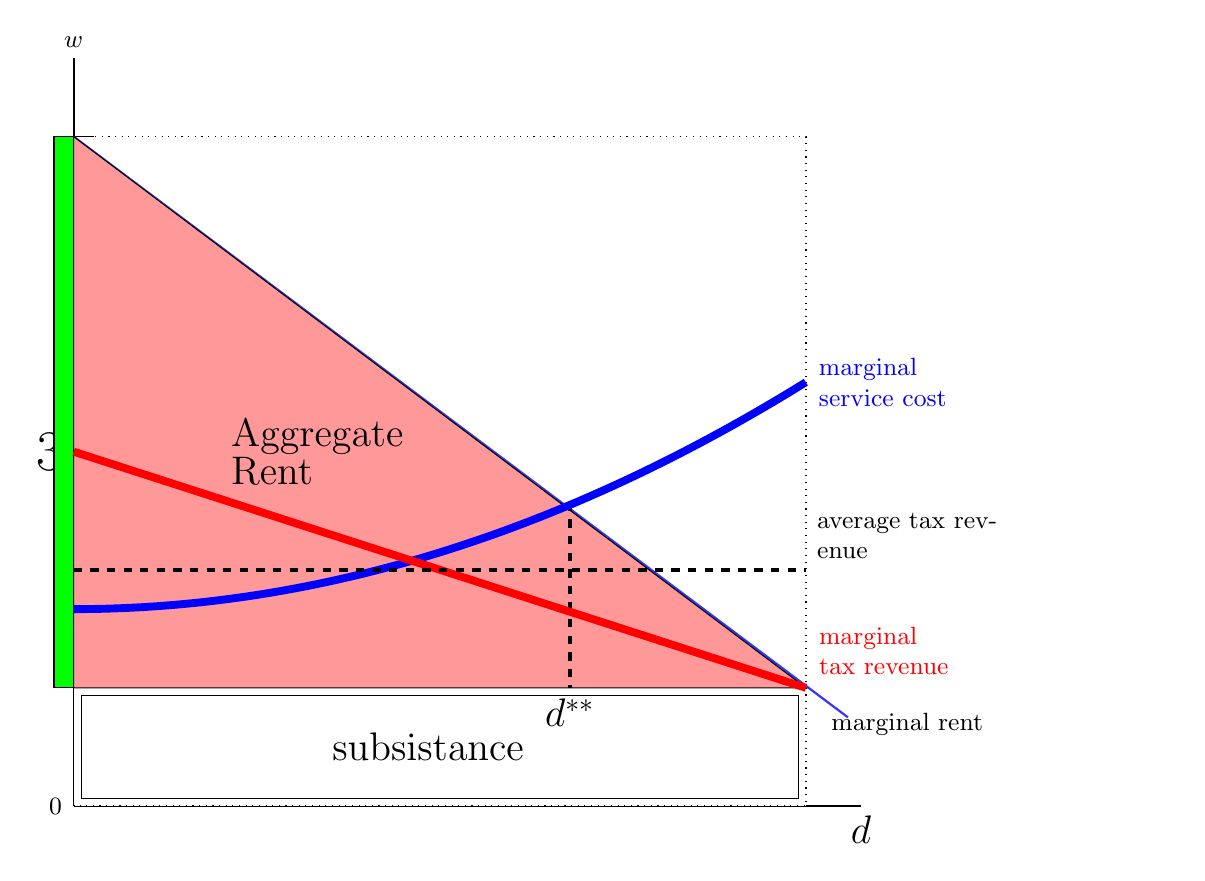
\begin{tikzpicture}[scale=1]
\def\bndmax{5}        %https://tex.stackexchange.com/questions/68462/filling-a-complex-region-with-tikz
\def\bndmin{0.2}
\def \n {8}  % height of y axis
\def \d {10}  % length  of x axis
\def \t {.75}  %  cost of transportation per unit x
\def \th {1}   %
\def \w {7}    %  wage premium
\def \om{1.5}%  omega =rural wage Zero for urban population
\def \azero{2}
\def \aprime {-.0}	
\tikzset{func/.style={thick,color=blue!80}}	
\draw [thick] (0,-\om) --(\d,-\om)node[below]{\Large$d$};  			% Zero for rural population
\draw [thick] (0,-\om)node[left=.5]{$0$} --(0,\n)node[above]{$w$};	% Y axis

%\draw [thick] (0,0)node[left=.5]{ subsistance}--(\d,0);
\node[left=.25] at (0,3){\huge $\omega$};
%\node[left=.25] at (0,\w+.3){subsistence plus};
%\node[left=.25] at (0,\w-.4){wage premium};	

\draw[fill=white, white] (0.1,-0.1) rectangle (14,-\om+.1);
\draw [fill=green] (-.25, 0) rectangle(.25, \w);
\node[right] at  (.25, \w/2){Added Productivity};
%\draw [ thick, ->](11.3,-\om/2)--(13, -\om/2)node [right] {\Large $d$};
\draw[fill=blue!40] (0.1,-0.1) rectangle (9.2,-\om+.1);


\draw[fill=black!0, dotted] (0,-\om) rectangle (9.30,\w);% new product repeat
\draw[func, domain=0:\w/\t+.5] plot [samples=200] (\x,{\w-\t*\x}); %rent profile
\draw[fill=blue!0] (0.1,-0.1) rectangle (9.2,-\om+.1);
\node at (4.5,-\om/2){\Large subsistance};
\draw[fill=red!40,] (0.,0.) -- (0,7)--(9.30,0.)--cycle;% Rent \w-.2
\node[text width=2cm] at (3.,3){\Large Aggregate \\Rent}; 		%Rent 
%\node at (5.8,5.7)[]{\Large Transportation};
\node at (6.3,4.8)[white]{\Large expenditure};
\draw[ line width=.5mm, dashed] (6.3,2.35)--(6.3,0)node[below ]{\Large$d^{**}$};

\draw[func, domain=0:9.3, line width=1mm,blue, text width=2cm] plot [samples=200] (\x,{1+\x^2/30})node[right]{marginal\\ service cost};
\draw[ line width=1mm, red] (0,3)--(9.3,0)node[above right, text width=3cm ]{marginal\\tax revenue};
\node at (9.5, -.2)[below right, text width=2cm]{marginal rent};

\draw[ line width=.5mm, dashed] (0,1.5)--(9.3,1.5)node[above right, text width=2.5cm ]{average tax revenue};

%GRID
%\draw[step=1cm,gray,very thin] (0,0) grid (10,10);


 \end{tikzpicture}
 
Two stylized facts should be noticed. The first is that the marginal cost of servicing generally  rises with the distance from the centre.  Figure~\ref{} illustrates the general form of servicing costs, but not  the relative scales of rent and servicing costs. When this observation is combined with the `Henry George Theorem" () the conclusion is that the optimal size of the city  is at  $d^{**}$, where marginal service cost intersects with the marginal increase in total urban rent. 


The second stylized fact  is that property taxes, which are generally  fixed as a share of property value, decline as the distance from the centre increases.Figure~\ref{} illustrates the general form of tax liabilities, although it does not  accurately represent their relationship top rent or  servicing costs.  This implies that in many or most urban situations the residents at the outer edges pay less than the average amount in property tax per unit of land, but cost  the community budget more than the average amount. In essence, the central city subsidizes the suburbs. (ref Perverse Cities}  This arrangement is both economically inefficient and unfair, but it has been built into the fiscal structure of cities largely as a result of automobile-based urban growth. It is likely that this fiscal misallocation saps some of the potential productivity growth of cities.

Both effects are more variable and than the simple model suggests.  One  conclusion urban theorists draw based on variants of the Alonzo model is that because property owners in the low-density urban margin are subsidized,  the subsidy is likely to create serious fiscal problems for municipalities in the long term and result in serious inefficiency in land use. 
